% fancytikzposter.tex, version 2.1
% Original template created by Elena Botoeva [botoeva@inf.unibz.it], June 2012
% 
% This file is distributed under the Creative Commons Attribution-NonCommercial 2.0
% Generic (CC BY-NC 2.0) license
% http://creativecommons.org/licenses/by-nc/2.0/ 


\documentclass{a0poster}
\usepackage{amsmath}
\usepackage{amsfonts}
\usepackage{fancytikzposter} 
\usepackage{wrapfig,kantlipsum}
%\usecolorstyle[RGB={110,200,22}]{bluedelft}
\setfirstcolor{blue!50!cyan}
\usepackage{color}
\definecolor{tuco}{RGB}{110, 200, 225}
\definecolor{backgroundcolorbottom}{RGB}{100,150,180}
\setbackgrounddarkcolor{white}
\setbackgroundlightcolor{backgroundcolorbottom}
\setblocktitlefillcolor{backgroundcolorbottom}
\settitledrawcolor{backgroundcolorbottom}
\setblocktitletextcolor{black}
%\setblocktextcolor{!30!black}
\setblocktitlefillcolor{tuco}
\setblocktitleheight{0.1}
\setblockspacing{0.0}
\setmargin{1.2}
\usepackage{tikz} 


%%% size of the document and the margins
%% A0
% \usepackage[margin=\margin cm, paperwidth=118.9cm, paperheight=84.1cm]{geometry} 
\usepackage[margin=\margin cm, paperwidth=84.1cm, paperheight=118.9cm]{geometry}
%% B1
% \usepackage[margin=\margin cm, paperwidth=70cm, paperheight=100cm]{geometry}



%% changing the fonts
\usepackage{cmbright}
%\usepackage[default]{cantarell}
%\usepackage{avant}
%\usepackage[math]{iwona}
\usepackage[math]{kurier}
\usepackage[T1]{fontenc}
\usepackage{color}
%% add your packages here
\usepackage{hyperref}
\usepackage{wrapfig,lipsum,booktabs}
\usepackage{amsmath}
\usepackage{amsfonts}
\usepackage{mathrsfs}
%\usepackage{cite}
\usepackage{graphicx}
\usepackage{float}
\usepackage[font=footnotesize]{caption}
\usepackage{subfigure}
\usepackage{pifont}




%\author[Diaz,Vuik,Jansen]
%{Gabriela Berenice Diaz Cortes  \\
 % Prof. Kees Vuik  \\ 
%Prof. J. D. Jansen\\ TU Delft }
\title{Physics-based preconditioners for large-scale subsurface flow simulation.}
\author{G. B. Diaz Cortes,
 C. Vuik,
J. D. Jansen\\
    
\includegraphics[width=0.2\textwidth]{TU_Delft_logo.png}
}%{
\includegraphics[]{flow1.jpg}}}
\usebackgroundtemplate{3}
\useblocknodetemplate{3}
%\useblocktitleheight{1}
\usetitletemplate{1}
%\titlegraphic{
\includegraphics[width=1cm,height=1cm]{flow1.jpg}}
%\hfill}

\begin{document}


%%%%% ---------- the background picture ---------- %%%%%
%% to change it modify the macro \BackgroundPicture
\ClearShipoutPicture
\AddToShipoutPicture{\BackgroundPicture}

\noindent % to have the picture right in the center
\begin{tikzpicture}

  \initializesizeandshifts
  % \setxshift{15}
   %\setyshift{2}


  %% the title block, #1 - shift, the default value is (0,0), #2 - width, #3 - scale
  %% the alias of the title block is `title', so we can refer to its boundaries later
  \ifthenelse{\equal{\template}{1}}{ 
    \titleblock{60}{0.8}{0.5}
  }

  %% a logo can be added to the title block
  %% #1 - anchor relative to the title block, #2 - shift, #3 - width, #3 - file name
   %\ifthenelse{\equal{\template}{2}}{ 
    % \addlogo[south west]{(2,0)}{6cm}{tulogo.png}
  % }{
  %   \addlogo[south west]{(2,0)}{6cm}{tulogo.png}
  % }


  %% a block node, with the specified position (optional), title and the content
  %% #1 - where (optional), #2 - title, #3 - text
  %%%%%%%%%% ------------------------------------------ %%%%%%%%%%
  \blocknode
  {Theory}%
  {\Large Linear System

    \coloredbox{colorone!50!}{
   \Large $$\mathbf{Ax}=\mathbf{b}.$$}
  \Large Iterative Methods.\\
  
   \coloredbox{colorone!50!}{\large
Initial guess solution $\mathbf{x}^0$, residual $\mathbf{r}^k=\mathbf{b}-\mathbf{Ax}^k$.

\Large Krylov subspace of dimension $k$.
$$\mathcal{K} _k(\mathbf{M}^{-1}\mathbf{A},\mathbf{M}^{-1}\mathbf{r}^0)=
span\{\mathbf{M}^{-1}\mathbf{r}^0,\dots,(\mathbf{M}^{-1}\mathbf{A})^{k-1}(\mathbf{M}^{-1}\mathbf{r}^0)\}.$$
}\\
Conjugate Gradient

\coloredbox{colorone!50!}{\Large
   

$$min_{\mathbf{x}^k \in \mathcal{K}_j (\mathbf{A},\mathbf{r}^0)}||x-\mathbf{x}^k||_\mathbf{A}, \qquad ||x||_\mathbf{A}:=\sqrt{(x,Ax).}$$ 
Iteration
$$\mathbf{x}^{k+1}=\mathbf{x}^k+\alpha_kp^k, \qquad \alpha^k=\frac{(\mathbf{r}^k,\mathbf{r}^k)}{(Ap^k,p^k)}, \qquad (Ap^i,p^j)=0, \text{ } i \neq j.$$ 

Convergence: \\
\coloredbox{colorone!0!}{
    $$ ||\mathbf{x}-\mathbf{x}^{k+1}||_\mathbf{A} \leq ||\mathbf{x}-\mathbf{x}^{0}||_\mathbf{A} \left( \frac{ \sqrt{\mathbf{C}(\mathbf{A})}-1}{\sqrt{\mathbf{C}(\mathbf{A})+1}} \right)^{k+1},$$\\ $$\text{ where } \mathbf{C}(\mathbf{\mathbf{A}}) 
    \text{ is the condition number of } \mathbf{\mathbf{A}}.$$}
}\Large
Preconditioning\\

   \coloredbox{colorone!50!}{
\large
The same solution of the original system, but a better spectrum.
$$\mathbf{M}^{-1}Ax=\mathbf{M}^{-1}\mathbf{b}$$

}
\Large Deflation \cite{Tang08}\\

\coloredbox{colorone!50!}{\large
Deflated System:
$$PA\hat{\mathbf{x}}=Pb, \qquad \hat{\mathbf{x}} \text{ is the deflated solution.}$$
$$\mathbf{x}=Qb+P^T\hat{\mathbf{x}}, \qquad \mathbf{x} \text{ is the solution of the original system}.$$
$$P=I-AQ,   \qquad Q=ZE^{-1}Z^T,\qquad P \in \mathbf{R}^{n \times n}, \qquad Q \in \mathbf{R}^{n \times n},$$
$$E=Z^TAZ, \qquad E \in \mathbf{R}^{k \times k}, \qquad Z \in \mathbf{R}^{n \times k}.$$
\\ \large Convergence (Deflation + Preconditioning): \\

\coloredbox{colorone!0!}{
\begin{equation*}
 ||\mathbf{x}-\mathbf{x}^{i+1}||_\mathbf{A}\leq 2||\mathbf{x}-\mathbf{x}^{0}||_\mathbf{A} \left( \frac{\sqrt{\mathbf{C}(\mathbf{M}^{-1}PA)}-1}{\sqrt{\mathbf{C}(\mathbf{M}^{-1}PA)}+1} \right)^{i+1}, \qquad \mathbf{C}(\mathbf{M}^{-1}PA)<\mathbf{C}(\mathbf{A}).
\end{equation*}
}
}
}
 \blocknode%
  {Proper Orthogonal Decomposition (POD) \cite{Mark06,Astrid11}}%
  {
\coloredbox{colorone!50!}{\large 
The POD
method is a ROM which basis functions are obtained from 'Snapshots' 
by simulation or experiment ,
  $$X:=[\mathbf{x}_1,\mathbf{x}_2,...\mathbf{x}_m], \qquad  \mathbf{x_i} \in \mathbf{R}^{n}.$$
The basis functions are a set of $l,$ $l\leq m << n,$ orthogonal vectors,  $\{ {\phi} _j \} ^l _{j=1},$ that correspond to the $l$ eigenvectors of the largest eigenvalues \Large $$
\frac{\sum_{j=1}^l\lambda_j}{\sum_{j=1}^m\lambda_j} \leq \alpha, \qquad 0<\alpha \leq 1,
$$  of 
the data snapshot correlation matrix,
$$
\mathbf{R}:= \frac{1}{m}\mathbf{X}\mathbf{X}^T \equiv \frac{1}{m} \sum_{i=1}^m \mathbf{x}_i \mathbf{x}_i^T.
$$}
}
  
  
  
%% a callout block
  %% #1 - rotate angle (optional), #2 - from, #3 - where, #4 - width, #5 - text
  %%%%%%%%%% ------------------------------------------ %%%%%%%%%%



  %%%%%%%%%% ------------------------------------------ %%%%%%%%%%  
  %\calloutblock{($(box.center)+(-10,-8)$)}
  %{($(box.center)+(10,-1)$)}
  %{19cm}
  %{
    %Convergence CG:
    %$$ ||x-x^{k+1}||_A \leq ||x-x{0}||_A \left( \frac{ %\sqrt{\kappa(A)}-1}{\sqrt{\kappa(A)+1}} \right)^{k+1}$$
 % }




  %%%%%%%%%%%%% NEW COLUMN %%%%%%%%%%%%%%% 
  \startsecondcolumn 

  %%%%%%%%%% ------------------------------------------ %%%%%%%%%%
   \blocknode%
  {Model}%
  {\large Single-Phase flow \\
\coloredbox{colorone!50!}{

The governing partial 
differential equations for single-phase flow result in a system of 
ordinary differential equations \cite{Jansen13}, 
$$
 \mathbf{V}\dot{\mathbf{p}}+\mathbf{T}\mathbf{p}=\mathbf{q},
$$
  
neglecting gravity and restricting the analysis to slightly compressible flow, the system is linear and
$\mathbf{p}$ is a vector of grid block pressures, $\mathbf{q}$ is a vector of grid block source terms (wells), 
the dot represents differentiation with respect to time, while $\mathbf{T}$ and 
$\mathbf{V}$ are the transmissibility and accumulation matrices.
We use the
Peaceman well model which gives: 
 \begin{equation*}\label{eq:peac}
  \mathbf{V}\dot{\mathbf{p}} + \mathbf{T}\mathbf{p} = \mathbf{J}(\mathbf{p}-\mathbf{p}_{well}),
\end{equation*}
where $\mathbf{J}$ is a matrix with well indices in the appropriate positions and $\mathbf{p}_{well}$ is a 
vector of well bore pressures \cite{Jansen13}. \\
For incompressible flow we have:
\begin{center}
\begin{minipage}{0.3\linewidth}
        
        \begin{equation*}
            \mathbf{T}\mathbf{p} = \mathbf{J}(\mathbf{p}-\mathbf{p}_{well}).
        \end{equation*}

      \end{minipage}
\end{center}

}
 %\begin{tikzfigure}[figura1] 
  %          
\includegraphics[width=0.4\textwidth]{flow1.jpg}
%\end{tikzfigure}\label{example_picture}
}

    
  \blocknode%
  {Snapshots as deflation vectors}%
  {\large


Heterogeneous permeability layers problem (4 snapshots)\\
\coloredbox{colorone!50!}{\large 
\begin{minipage}{.4\textwidth}
\centering
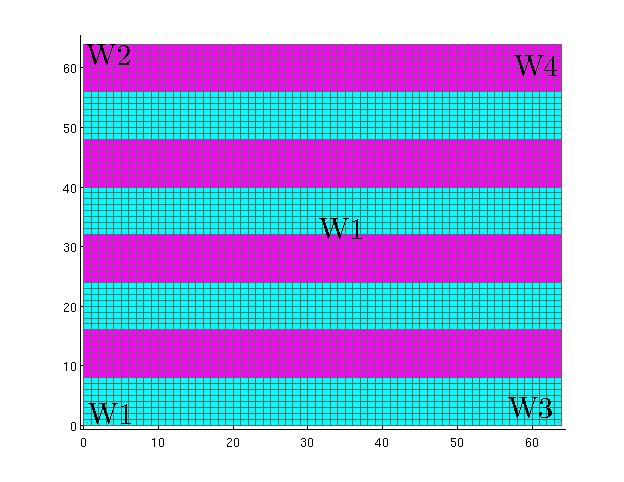
\includegraphics[width=10cm,height=10cm,keepaspectratio]{perm_he_2.jpg}
\end{minipage}%
\begin{minipage}{.5\textwidth}
\vspace{1.5cm}
\begin{center}
\begin{tabular}{ |c|c|c|} 
\hline
 $\kappa_2$ (mD) & $10^{-1}$& $10^{-3}$ \\
 \hline
  ICCG  & 75& 110\\ 
  DICCG  & 1 & 1\\ 
 \hline
\end{tabular}
\end{center}
\normalsize
Number of iterations for the ICCG and DICCG methods ($tol =10^{-11}$), varying permeability contrast between layers .
\end{minipage}}
\large
SPE10 (2nd layer, 4 snapshots)\\
\\
\coloredbox{colorone!50!}{\large 
\begin{minipage}{.45\textwidth}

\begin{center}
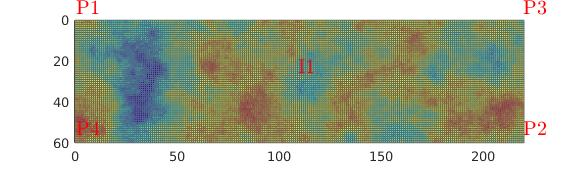
\includegraphics[width=16cm,height=14cm,keepaspectratio]{perm_2layer.jpg}
\end{center}
\end{minipage}%
\begin{minipage}{.5\textwidth}
\vspace{2cm}
\begin{center}
\begin{tabular}{|c|c|c|c|c|  } 
 \hline
Method  & 16x56 & 30x110 & 46x166 & 60x220\\
  \hline
  ICCG                & 34 & 73&  126&  159\\ 
   \hline
DICCG & 1 & 1&  1 &  1 \\ 
\hline
\end{tabular}
\end{center}
\normalsize
Number of iterations for ICCG and DICCG methods ($tol =10^{-11}$),
various grid sizes.
\end{minipage}}

}
  
  \blocknode%
  {POD-based deflation vectors}%
  {\large SPE10 (15 snapshots)\\
  \coloredbox{colorone!50!}{\large 
  \begin{minipage}{.45\textwidth}
  \large
\begin{center}
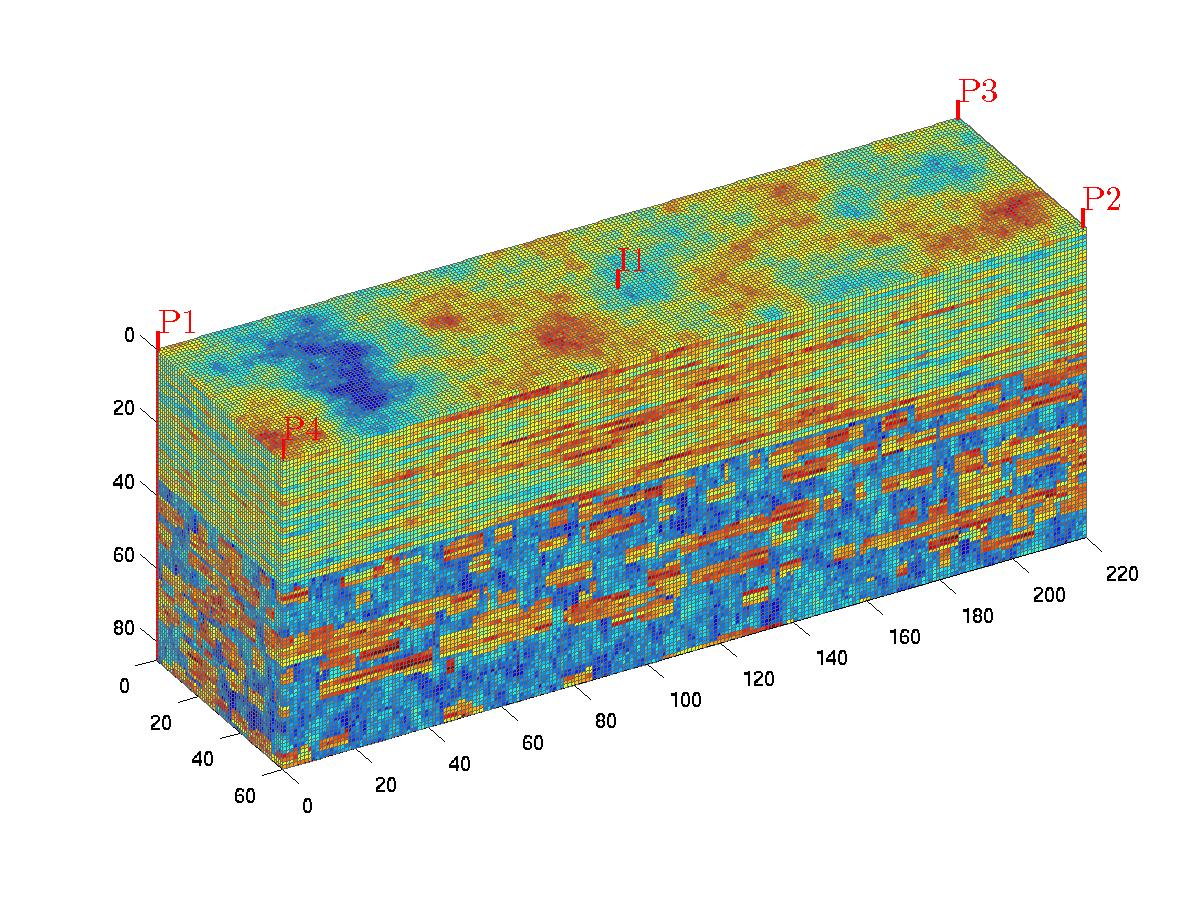
\includegraphics[width=16cm,height=16cm,keepaspectratio]{perm_layer_.jpg}
\end{center}
\end{minipage}%
\begin{minipage}{.5\textwidth}
\vspace{2cm}
\begin{center}
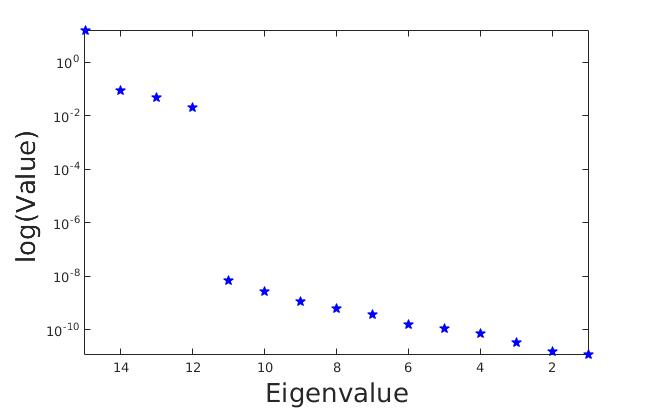
\includegraphics[width=15cm,height=15cm,keepaspectratio]{eig_pod_l.jpg}
\end{center}
\normalsize
Eigenvalues of 15 snapshots obtained with ICCG ($tol= 10^{-11}$).
\end{minipage}

\centering
\begin{minipage}{.5\textwidth}
\vspace{1cm}
\begin{center}
\begin{tabular}{ |c|c|} 

 \hline
 Method & Iterations\\
 \hline
  ICCG  & 1011\\ 
  \hline
  DICCG$_{15}$  & 2000 \\ 
  \hline
  DICCG$_{POD}$ & 2\\
 \hline
\end{tabular}
\end{center}
\normalsize
Number of iterations
for the ICCG, DICCG$_{15}$ and DICCG$_{POD}$ methods, tolerance of solvers and snapshots $10^{-11}$. 
\end{minipage}}

 }

\blocknode{}{\small
\bibliographystyle{unsrt}
\bibliography{research}
}


\end{tikzpicture}



\end{document}




